\def\relativepath{BiPart/} % ← chemin relatif depuis le main

\graphicspath{{\relativepath Figures/}} % pour les images
\makeatletter
\def\inputfile#1{\input{\relativepath#1}} % pour les sous-fichiers
\makeatother

\makeatletter
\let\oldinput\input
\def\input#1{\oldinput{\relativepath#1}}
\makeatother

% Utilisation :
%\inputfile{texte.tex}
%\includegraphics[width=\textwidth]{image1.png}



%\chapter{Quench bipartite dans un gaz de Bose unidimensionnel}

\section*{Introduction}%Dans ce chapitre, nous étudions l’évolution d’un gaz quantique unidimensionnel après une rupture de symétrie initiale. Nous utilisons un gaz de bosons ultra-froids, confiné dans une géométrie unidimensionnelle. Ce gaz est décrit par le modèle intégrable de Lieb-Liniger. Les interactions entre atomes sont faibles et répulsives.

%Nous préparons d’abord un gaz homogène (Fig \ref{fig:BiPart.insitut}). Ensuite, nous supprimons brutalement une moitié du nuage. Cela crée une frontière nette entre deux zones : une avec des atomes , l’autre vide (Dans notre protocole la partie sans des atomes se trouve en $x<0$ et avec atomes en $x>0$) (Fig \ref{fig:BiPart.coupure1} (a),(b),(c),(d)). Cette configuration correspond à ce qu’on appelle un « quench bipartite ».


%\begin{figure}[H]
%	\centering
%	\begin{subfigure}[b]{0.3\textwidth}
%		\begin{tikzpicture}
%			\begin{scope}[shift={(2,0)}]
%				\begin{scope}[transform canvas={scale=0.6}]
					%% Définition des couleurs avec les codes HTML
\definecolor{colorOne}{HTML}{443E46}
\definecolor{colorTwo}{HTML}{F6DEB8}
\definecolor{colorThree}{HTML}{908CA4}
\definecolor{colorFour}{HTML}{57659E}
\definecolor{colorFive}{HTML}{C57284}
\definecolor{colorSix}{HTML}{FF5B69}

% Raccourcis pour les couleurs
\def\colorOne{colorOne}
\def\colorTwo{colorTwo}
\def\colorThree{colorThree}
\def\colorFour{colorFour}
\def\colorFive{colorFive}
\def\colorSix{colorSix}

\def\colorslide{blue!50!black}



\begin{scope}
	% Tracer une courbe lisse entre des points
	\draw[shift={(0,0)} ,\colorOne]
		(-1 , 0 ) edge [thick,line width=0.8ex , ->,>=triangle 45  , \colorOne] node [pos = 1 , below ]{\huge$\rho$}( 5  , 0 )
	;
	\draw[shift={(0,0)}, color=\colorOne]
		(0, -1.0 ) edge [thick,line width=0.8ex , ->,>=triangle 45  ]node [pos=0.9,left=0.2cm ]{\huge$\mathcal{A}(\rho)$}( 0  , 5 )
	;
	\draw[]
		(2.5, 0.12 ) edge [thick,line width=0.8ex ,\colorThree ]node [pos=1,below  ]{\huge$\rho^c$} (2.5, -0.12 )	
	;
	
	\draw[]
		(2.5, -0.12 ) edge [thick,line width=0.4ex , dashed, \colorThree ] (2.5, 5.5 )
		(1.5, 1 ) edge [thick,line width=0.4ex , <->,>=triangle 45  , \colorThree ] (3.5, 1 )
		(-0.3,1) edge [thick,line width=0.4ex  , \colorThree ] node [pos=0,left ]{\huge$\mathcal{A}(\rho^c)$} (0.3, 1 )	
	;
    \draw[thick, line width=0.8ex , \colorFour] plot[smooth, tension=0.7] coordinates {
        (1, 5) (1.6 , 3 ) (2.5, 1) (3.5 , 3 )  (4, 5)
    };		
	
\end{scope}

	
			
%				\end{scope}
			
%				\draw[color = red , scale = 0.5 , draw = none  ] (-2 , -1) rectangle (5, 6) ; 	
%			\end{scope}
					
%		\end{tikzpicture}
%		\caption{}
%		\label{fig:grap.A}
%	\end{subfigure}
%	\hfill
%	\begin{subfigure}[b]{0.65\textwidth}
%		\begin{tikzpicture}

%			\begin{scope}[shift={(-11,2.7)}]
%				\begin{scope}[transform canvas={scale=0.6}]
					%% Définition des couleurs avec les codes HTML
\definecolor{colorOne}{HTML}{443E46}
\definecolor{colorTwo}{HTML}{F6DEB8}
\definecolor{colorThree}{HTML}{908CA4}
\definecolor{colorFour}{HTML}{57659E}
\definecolor{colorFive}{HTML}{C57284}
\definecolor{colorSix}{HTML}{FF5B69}

% Raccourcis pour les couleurs
\def\colorOne{colorOne}
\def\colorTwo{colorTwo}
\def\colorThree{colorThree}
\def\colorFour{colorFour}
\def\colorFive{colorFive}
\def\colorSix{colorSix}

\def\colorslide{blue!50!black}

\def\Occupation{
	\def\traitx{0.3}
	\def\traity{0.5}
	\draw[shift={(0,0)}]
		(-13.5 , 0 ) edge [thick,line width=0.8ex ]( -3.2  , 0 )
		( -3.2 - \traitx  , 0 - \traity ) edge [thick,line width=0.8ex ]( -3.2 + \traitx  , 0 + \traity  )
		( -2.8 - \traitx  , 0 - \traity ) edge [thick,line width=0.8ex ]( -2.8 + \traitx  , 0 + \traity  )
		(-2.8 , 0 ) edge [thick,line width=0.8ex ](2.8  , 0 )
		( 2.8 - \traitx  , 0 - \traity ) edge [thick,line width=0.8ex ]( 2.8 + \traitx  , 0 + \traity  )
		( 3.2 - \traitx  , 0 - \traity ) edge [thick,line width=0.8ex ]( 3.2 + \traitx  , 0 + \traity  )
		(3.2, 0 ) edge [thick,line width=0.8ex,->,>=triangle 45 , color = black ]node [pos=1.01,below  ]{\huge$\theta$}	( 13  , 0 )
	;
	\draw[shift={(0,0)}, color=\colorOne]
		(-10.5 , -1.5 ) edge [thick,line width=0.8ex , ->,>=triangle 45  ]( -10.5  , 4.5 )
	;
		
	\foreach \r in {1 , ... , 3 } {
%		\draw[
%		decoration={
%		markings,
%    	mark connection node=my node,
%    	mark=at position 0 with{\node [blue,transform shape] (my node) {\large \r};}},
%		color=gray, thick, 
%		line width=0.5ex] decorate { 
%            (-11.0, \r) -- (-10.1, \r )}
%        ;
        \draw[
			color=\colorOne,
			] 
            (-11.0, \r) edge[color=\colorThree , thick,line width=0.5ex] node [pos=-0.5 ]{\large\color{\colorFour} $\frac{\r}{\delta \theta}$ } (-10.3, \r )
        	;
	
	}
	

	
	% Graduation abcsisse 
	% Définitions des listes
% Definitions of the lists
\def\listetuple{-9/\theta_{1}, -8/\theta_{2} , -5/\theta_{3} , -2/\theta_{a-1} , 0/\theta_{a} , 1/\theta_{a+1} , 2/\theta_{a+2} ,  5/\theta_{N-4} , 7/\theta_{N-3},8/\theta_{N-1},9/\theta_{N} }
\def\listetrais{-12 , -11, -10, -9 , -8 , -7 ,  -6 , -5, -4.5,-4, -2 , -1, 0 , 0.5, 1, 2, 4 , 5 ,  6 , 7 , 8 ,8.5, 9 ,  10 , 11, 12 }

% Loop over listetrais
\foreach \r in \listetrais {
    % Initialize found variable to zero
    % Initialize found variable to zero
    %\pgfmathsetmacro\found{0}
    \global\def\found{0}
    \xdef\nomtheta{}
    
    % Check if \r is in listetuple
    \foreach \x/\y in \listetuple { 
        \ifdim \r pt=\x pt % If \r matches any \x in listetuple
            \global\def\found{1} ;
            \xdef\nomtheta{\y} % Set \nomtheta to the corresponding \y
            %\pgfmathsetmacro\found{1} % Set found to 1            
            %\global\pgfmathsetmacro\found{1}
        \fi
    }
    
    %\node [circle, draw, red] (A) at (\r, 2) {\found , $\nomtheta$};
    
    % Draw the line and display \nomtheta if found
    \ifnum\found=1
        \draw[color=\colorOne, thick, line width=0.5ex] 
            (\r, -0.3) -- (\r, 0.3) node[red , pos=-0.5] {\large $\nomtheta$};
         \filldraw[line width=0.5ex, color=\colorSix, outer color=\colorSix, inner color=\colorSix] 
            (\r, 0) circle (4pt);
    \else 
        % Draw without \nomtheta and add a blue circle if not found
        \draw[color=\colorOne, thick, line width=0.5ex] 
            (\r, -0.3) -- (\r, 0.3);
        \filldraw[line width=0.5ex, color=\colorSix, outer color=\colorTwo, inner color=\colorTwo] 
            (\r, 0) circle (4pt); 
    \fi
}

\def\listetrais{-9.5/\theta_{i-1}/2/3, -6.5/\theta_{i}/1/4  ,   -1.5/\theta_{j}/2/4 , 1.5/\theta_{j+1}/-1/3 , 3.5/\theta_{\ell-1}/1/3 , 6.5/\theta_{\ell}/3/4 , 9.5/\theta(\theta_{\ell+1})/-1/3 };



\foreach \r/\nomx/\y/\ys in \listetrais {
	\draw[
		decoration={
		markings,
    	mark connection node=my node,
    	mark=at position .5 with{\node [blue,transform shape] (my node) {\large \color{\colorFour} $\nomx$};}},
		color=\colorThree , thick, 
		line width=0.5ex] decorate { 
            (\r, 0.12) -- (\r, -1.2)}
        ;
     
     \ifdim \y pt > -1 pt 
     	\draw[
			decoration={
			markings,
    		mark connection node=my node,
    		mark=at position .5 with{\node [blue,transform shape] (my node) {\large \color{\colorFour} $\Pi(\nomx) $};}},
			color=\colorThree, thick, 
			line width=0.5ex] decorate { 
            (\r, \y) -- (\r +3, \y)}
        ;
        \draw[
			decoration={
			markings,
    		mark connection node=my node,
    		mark=at position .5 with{\node [blue,transform shape] (my node) {\large \color{\colorFive} $\Pi_s(\nomx) $};}},
			color=\colorFive, thick, 
			line width=0.5ex] decorate { 
            (\r, \ys) -- (\r +3, \ys)}
        ;
     \fi 
     \ifdim \r pt= -1.5 pt
     	\draw[
     		decoration={
			markings,
    		mark connection node=my node,
    		mark=at position .5 with{\node [blue,transform shape] (my node) {\large \color{\colorFour}  $\delta \theta $};},
    		%mark=at position 0.1  with {\arrow[blue, line width=0.5ex]{<}},
    		%mark=at position 1  with {\arrow[blue, line width=0.5ex]{>}}
    		},
        	color=\colorThree,
        	thick,
        	line width=0.5ex,
        	%arrows={Computer Modern Rightarrow[line cap=round]-Computer Modern Rightarrow[line cap=round]}
   			](\r, -1.2) edge[arrows={Computer Modern Rightarrow[line cap=round]-}] (\r + 0.4, -1.2)decorate {
    		(\r, -1.2) -- (\r + 3, -1.2)}(\r + 2, -1.2) edge[arrows={-Computer Modern Rightarrow[line cap=round]}] (\r + 3, -1.2)
    		;
    \fi
			
	
}


			
}


\begin{scope}
	%\draw[help lines , width=1.5ex] (-8,-3) grid (8,3);\draw[help lines ,width=0.5ex , opacity = 0.5] (-3,-3) grid[step=0.1] (3,3));
	
	%\draw[help lines] 
	%	(-3,-3) edge[width=1.5ex] grid (3,3)	
	%	(-3,-3) edge[width=0.5ex , opacity = 0.5] grid (3,3)	
	%;
	\begin{scope}[shift={(0,1)},rotate=0,opacity=1,color=black]
		\Occupation	
		
		%\node[anchor=east, font=\bfseries] at (-11, 0) {\color{red}\large (T = 0 )} ;	
	\end{scope}
	
	
	
	
	\begin{scope}[shift={(-10.5,7)},rotate=0,opacity=1,color=black]
	
	\begin{scope}[shift={(-0,0)},rotate=0,opacity=1,color=black]
	
		\draw[shift={(0,0)} ,line width=1ex,rounded corners = 1ex,color=\colorOne , opacity =1 ,fill=\colorOne!00 , pattern={north east lines} , pattern color=\colorOne!00 ]
			(0 , -1 ) rectangle (5,1)
		;
		

		\begin{scope}[shift={(0.5,0.5)}]
			\draw[color=\colorOne, thick, line width=0.5ex] 
            (0, -0.3) -- (0, 0.3) ;
            \filldraw[line width=0.5ex, color=\colorSix, outer color=\colorSix, inner color=\colorSix] 
            (0, 0) circle (4pt);
            
            \node[anchor=west, font=\bfseries] at (0.2, 0) {\color{\colorSix}\large : quasi-particule};
		\end{scope}
		
		\begin{scope}[shift={(0.5,-0.5)}]
			\draw[color=\colorOne, thick, line width=0.5ex] 
            (0, -0.3) -- (0, 0.3) ;
            \filldraw[line width=0.5ex, color=\colorSix, outer color=\colorTwo, inner color=\colorTwo] 
            (0, 0) circle (4pt);
            
            \node[anchor=west, font=\bfseries] at (0.2, 0) {\color{\colorSix}\large : hole};
		\end{scope}

	\end{scope}
	
	\begin{scope}[shift={(6,0)},rotate=0,opacity=1,color=black]	
		
		\draw[shift={(0,0)} ,line width=1ex,rounded corners = 1ex,color=\colorOne , opacity =1 ,fill=\colorOne!00 , pattern={north east lines} , pattern color=\colorOne!00 ]
			(0 , -1 ) rectangle (7.5,1)
		;
		
		\node[anchor=west] at (0.5, 0.5) {\color{\colorFour}\large $\Pi$ };\node[anchor=west, font=\bfseries] at (1, 0.5) {\color{\colorFour}\large : quasi-particule distribution};
		
		\node[anchor=west] at (0.5, -0.5) {\color{\colorFour}\large $\Pi_h$ };\node[anchor=west, font=\bfseries] at (1, -0.5) {\color{\colorFour}\large  : hole distribution};
		
	\end{scope}
	
	\begin{scope}[shift={(14.5,0)},rotate=0,opacity=1,color=black]	
		
		\draw[shift={(0,0)} ,line width=1ex,rounded corners = 1ex,color=\colorOne , opacity =1 ,fill=\colorOne!00 , pattern={north east lines} , pattern color=\colorOne!00 ]
			(0 , -0.5 ) rectangle (7.0,0.5)
		;
		
		\node[anchor=west] at (0.2, 0) {\color{\colorFour}\large ${\color{\colorFive}\Pi_s} = \Pi + \Pi_h $ } node[anchor=west , font=\bfseries] at (3.1 , 0 )  {\color{\colorFour}\large {\color{\colorFive} : density of states}};
		
	\end{scope}
	
	
	\end{scope}


		
	
\end{scope}

	
			
%				\end{scope}
%				\begin{scope}[scale=1]
%					\draw[color = red , scale = 1 , draw = none  ] (-1 , -1) rectangle (5, 5) ; 
%				\end{scope}	
%			\end{scope}
			
%		\end{tikzpicture}
%		\caption{}
%		\label{fig.fluctu.A}
%	\end{subfigure}
%	\caption{}
%	\label{fig:diag_fig}
%\end{figure}


%Le gaz évolue ensuite selon la dynamique de son Hamiltonien. Nous observons le déplacement de la frontière au cours du temps. Pour cela, nous mesurons le profil de densité atomique à différents temps d’évolution.

%Nous voyons que la frontière se propage de manière balistique. La largeur du profil de densité augmente de façon linéaire avec le temps. Ce comportement est prédit par la théorie de l’hydrodynamique généralisée (GHD). Cette théorie décrit comment les propriétés locales d’un système intégrable évoluent dans le temps (Fig \ref{fig:BiPart.coupure1} (e),(f),(g)). %Elle repose sur une distribution appelée « distribution de rapidité ». Cette fonction décrit la répartition des quasi-particules dans le système.

%Dans notre cas, GHD prévoit un profil de densité particulier si le gaz initial est à température nulle. Les données expérimentales sont proches de cette prédiction, mais avec de légers écarts. Ces écarts peuvent venir de la température non nulle du gaz ou d’autres imperfections expérimentales.

%Nous montrons que le profil de densité contient beaucoup d’informations. En théorie, on peut retrouver la distribution de rapidité initiale à partir du profil de frontière. Cela permettrait d’avoir une méthode d’analyse très puissante, comme une sorte de « thermomètre généralisé ». %Cependant, cette méthode est sensible au bruit dans les données, surtout dans les parties du profil où la densité est très faible. Pour contourner cela, nous utilisons un modèle simple avec trois paramètres pour approximer la distribution de rapidité. Ce modèle donne de bons résultats et reste plus robuste.

%Enfin, nous utilisons une nouvelle méthode expérimentale pour mesurer la distribution de rapidité localement (Part {??}) , à l’intérieur du profil. Nous observons une asymétrie, comme prévu par la théorie. D’un côté, la distribution est lisse et large ; de l’autre, elle est plus abrupte, comme pour un état fondamental. Cette observation confirme le comportement prédictif de la GHD, bien que la résolution spatiale limite la finesse des détails que nous pouvons observer.


%Parmi les systèmes à N corps, les modèles intégrables occupent une place particulière, notamment dans le contexte des dynamiques hors d’équilibre et de la thermalisation généralisée. Contrairement aux systèmes génériques, ces modèles présentent une infinité de constantes du mouvement, empêchant la thermalisation au sens habituel. Cela conduit à l’émergence d’une thermalisation généralisée, décrite non par l’ensemble canonique, mais par une ensemble à entropie maximale sous contraintes — souvent formalisé par l’Ensemble de Gibbs Général (GGE) \index{Ensemble Thermodynamique Général (GGE)}\index[pers]{Ensemble Thermodynamique Général (GGE), Ensemble de Gibbs Général (GGE)}.

%Un exemple pédagogique pour appréhender cette dynamique non triviale est fourni par l’expérience du pendule de Newton : des chocs élastiques entre sphères de masses égales illustrent parfaitement l’absence de thermalisation, l'énergie cinétique se propageant de manière cohérente entre les particules. Cette dynamique régulière, bien que classique, annonce les comportements typiques des systèmes intégrables quantiques où les excitations se déplacent sans diffusion.

%Dans ce cadre, le problème de Riemann en hydrodynamique — c’est-à-dire l'évolution d’un système à partir de deux états homogènes initiaux juxtaposés — fournit un test fondamental de compréhension des équations d’évolution des systèmes intégrables. Longtemps restée partiellement ouverte, la résolution complète de ce problème dans les modèles intégrables quantiques a été obtenue grâce à la formulation de la Théorie Hydrodynamique Généralisée (GHD).

%La GHD a été introduite dans [60] pour des théories des champs intégrables (comme le modèle de Sinh-Gordon ou le modèle de Lieb-Liniger décrivant un gaz de bosons 1D en interaction), et dans [59] pour les chaînes quantiques, notamment la chaîne XXZ anisotrope de Heisenberg. Ces travaux ont permis de résoudre analytiquement le problème de Riemann dans des systèmes quantiques fortement corrélés.

%Depuis, des solutions analytiques ont été obtenues pour des cas spécifiques. En particulier, une solution exacte du problème de Riemann pour la chaîne XXZ a été trouvée pour un état initial particulier [179]. Par ailleurs, une solution plus générale a été obtenue pour un gaz 1D de sphères dures, mettant en lumière l’efficacité de la GHD à capturer les phénomènes de propagation balistique et de relaxation généralisée dans un cadre quantique.

%%%%%


%Dans ce chapitre, nous étudions la dynamique hors équilibre d’un gaz quantique unidimensionnel de bosons faiblement interactifs, préparé dans un état initial présentant une rupture abrupte de symétrie. Le système est décrit par le modèle intégrable de Lieb-Liniger, et sa dynamique unitaire est analysée dans le cadre de l’hydrodynamique généralisée (GHD), un formalisme théorique développé récemment pour capturer l’évolution spatio-temporelle des observables locales dans les systèmes quantiques intégrables.

%Le protocole expérimental consiste en un "quench bipartite" : le gaz initial, homogène et à densité constante, est brutalement tronqué, de sorte que la moitié gauche du système ($x<0$) est vidée, tandis que la moitié droite ($x>0$) reste occupée (Fig.~\ref{fig:BiPart.coupure1}). Cette configuration induit une discontinuité initiale dans le facteur d’occupation $\nu(x,\theta)$, menant à une situation analogue au problème de Riemann dans les systèmes à un nombre infini de lois de conservation. Ce type de dynamique, souvent qualifié de domain wall dynamics, a été étudié en détail dans la thèse de Léa Dubois \cite{DuboisThese}, où une première analyse expérimentale de ce protocole a été réalisée.

%Dans ce travail, nous approfondissons cette étude en mettant l’accent sur la modélisation théorique fine à l’aide des outils de la GHD. Plus précisément, nous montrons que la propagation balistique observée de la discontinuité est bien décrite par la solution GHD du problème de Riemann, à température nulle comme finie. Nous analysons quantitativement les profils de densité mesurés expérimentalement et discutons en détail les écarts observés avec les prédictions théoriques idéales, en lien avec les effets thermiques et les imperfections instrumentales.

%Un point central de notre étude consiste à exploiter les solutions GHD pour reconstruire la distribution de rapidités initiale à partir du profil de densité mesuré dans la région de transition. Cette approche, que l’on peut interpréter comme une forme de thermométrie généralisée, constitue une méthode puissante pour sonder les états locaux du gaz. Nous mettons également en œuvre une nouvelle méthode expérimentale permettant de mesurer localement le facteur d’occupation $\nu(x,\theta)$ dans la région de déformation, mettant en évidence une forte asymétrie entre les deux côtés de la discontinuité, signature de la nature hors équilibre du système.


%%%%
%Dans ce chapitre, nous étudions la dynamique hors équilibre d’un gaz quantique unidimensionnel suite à une rupture initiale de symétrie. Le système étudié est un gaz de bosons ultra-froids confiné dans une géométrie unidimensionnelle, dont la dynamique est décrite par le modèle intégrable de Lieb-Liniger. Les interactions interatomiques sont faibles et de nature répulsive, ce qui permet d’explorer un régime faiblement corrélé tout en conservant des effets quantiques collectifs non triviaux.\\

%La préparation initiale consiste en un gaz homogène à profil de densité uniforme (Fig.~\ref{fig:BiPart.insitut}). Une opération de coupe abrupte est ensuite réalisée, supprimant spatialement la moitié gauche du nuage atomique. Il en résulte une condition initiale présentant une discontinuité marquée : la région $x<0$ est vide, tandis que des atomes occupent la région $x>0$ (Fig.~\ref{fig:BiPart.coupure1} (a)-(d)). Cette configuration correspond à un quench bipartite, c’est-à-dire une mise hors équilibre induite par une discontinuité initiale dans la densité.


%Après la préparation initiale, le gaz évolue selon la dynamique unitaire régie par son Hamiltonien. Pour suivre cette évolution, nous mesurons le profil de densité atomique à différents temps, ce qui permet de visualiser la propagation de la discontinuité initiale.

%Nous observons que la frontière entre les régions occupée et vide se propage de manière balistique : la largeur du profil de densité croît linéairement avec le temps. Ce comportement est en accord avec les prédictions de la théorie de l’hydrodynamique généralisée (GHD), qui fournit une description efficace de l’évolution spatio-temporelle des observables locales dans les systèmes intégrables (Fig.~\ref{fig:BiPart.coupure1} (e)-(g)).\\



%Dans notre configuration, la théorie de l’hydrodynamique généralisée (GHD) prédit un profil de densité caractéristique dans le cas d’un gaz initial à température nulle. Les mesures expérimentales obtenues sont globalement en accord avec cette prédiction, bien qu’on observe de légers écarts. Ces déviations peuvent être attribuées à une température initiale non nulle, ainsi qu’à d’éventuelles imperfections expérimentales.

%Nous montrons que le profil de densité contient une richesse d’information sur l’état initial du système. En particulier, la théorie suggère qu’il est, en principe, possible de reconstruire la distribution de rapidité initiale à partir du profil mesuré au niveau de la frontière. Cela ouvre la voie à une méthode d’analyse puissante, que l’on peut interpréter comme une forme de thermomètre généralisé dans le cadre de la GHD.\\

%Enfin, nous mettons en œuvre une nouvelle méthode expérimentale permettant de mesurer localement la distribution de rapidité au sein du profil de densité (voir Partie {??}). Nous observons une asymétrie marquée dans la forme de cette distribution : d’un côté, elle est large et lisse, tandis que de l’autre, elle présente une coupure abrupte, caractéristique d’un état proche du fondamental. Cette observation est en accord avec les prédictions théoriques de la GHD, bien que la résolution spatiale de notre dispositif limite la précision des détails accessibles.
\begin{figure}[!htb]
	\centering
	\includegraphics[width=0.5\textwidth , page = 4 ]{Shema.pdf}	
	%\caption{a) Facteur d'occupation initial $\nu(x, \theta) = \nu_0(\theta)$ correspondant à l'équilibre thermique à la température $T = 560~\mathrm{nK}$, pour une densité spatiale linéique $n_0 = 56~\mu\mathrm{m}^{-1}$, soit une potentielle chimique $\mu = 65~\mathrm{nK}$.  
%(b) Densité spatiale linéique $n(x) = \int \rho_{[\nu]}(x, \theta)\, d\theta \equiv n_0 = 56~\mu\mathrm{m}^{-1}$.  
%(c) Facteur d'occupation initial $\nu_0(\theta)$ correspondant au cas présenté en a).}
	\caption{a) Facteur d’occupation initial $\nu(x, \theta) = \nu_0(\theta)$ correspondant à un état d’équilibre thermique à la température $T = 560~\mathrm{nK}$, pour une densité linéique homogène $n_0 = 56~\mu\mathrm{m}^{-1}$. Ces paramètres correspondent à une potentielle chimique $\mu = 65~\mathrm{nK}$.
b) Densité spatiale linéique $n(x) = \int \rho_{[\nu]}(x, \theta), d\theta$, constante et égale à $n_0 = 56~\mu\mathrm{m}^{-1}$.
c) Facteur d’occupation $\nu_0(\theta)$ correspondant à la distribution thermique illustrée en a).}
	\label{fig:BiPart.insitut}
\end{figure}


Parmi les systèmes à N corps, les modèles intégrables occupent une place particulière, notamment dans le contexte des dynamiques hors d’équilibre et de la thermalisation généralisée. Contrairement aux systèmes génériques, ces modèles présentent une infinité de constantes du mouvement, empêchant la thermalisation au sens usuel. Cette contrainte conduit à l’émergence d’une thermalisation généralisée, décrite non par l’ensemble canonique, mais par un ensemble à entropie maximale sous contraintes, souvent formalisé par l’Ensemble de Gibbs Général (GGE) \index{Ensemble Thermodynamique Général (GGE)}\index[pers]{Ensemble Thermodynamique Général (GGE), Ensemble de Gibbs Général (GGE)}.

Un exemple classique pour illustrer la dynamique non diffusante typique des systèmes intégrables est celui du pendule de Newton, où des chocs élastiques entre sphères de masses égales propagent l’énergie cinétique sans dissipation. Bien que ce système soit classique, il incarne le comportement régulier que l’on retrouve dans les systèmes intégrables quantiques, où les excitations se déplacent sans diffusion.

Dans ce cadre, le problème de Riemann en hydrodynamique — c’est-à-dire l’évolution d’un système à partir de deux états homogènes juxtaposés — constitue un test fondamental de compréhension des équations d’évolution dans les systèmes intégrables. Sa résolution complète, longtemps restée partiellement ouverte, a été rendue possible par l’avènement de la Théorie Hydrodynamique Généralisée (GHD). Introduite dans le contexte des théories des champs intégrables (modèle de Sinh-Gordon, modèle de Lieb-Liniger) [??] et des chaînes quantiques (chaîne XXZ de Heisenberg) [??], la GHD a permis une avancée analytique majeure pour la description des dynamiques hors équilibre dans ces systèmes.

Depuis, plusieurs solutions analytiques du problème de Riemann ont été obtenues. En particulier, une solution exacte pour un état initial particulier dans la chaîne XXZ [??], ainsi qu’une solution plus générale pour un gaz 1D de sphères dures, ont confirmé l’efficacité de la GHD pour décrire les processus de propagation balistique et de relaxation généralisée.

Dans ce contexte, nous étudions la dynamique hors équilibre d’un gaz quantique unidimensionnel de bosons faiblement interactifs, confinés dans une géométrie 1D. Le système est décrit par le modèle intégrable de Lieb-Liniger, avec des interactions faibles et répulsives permettant l’émergence d’effets quantiques collectifs tout en restant dans un régime faiblement corrélé.

La préparation initiale consiste à créer un gaz homogène à profil de densité constant (Fig.\ref{fig:BiPart.insitut}), à température contrôlée. Une opération de coupe abrupte est ensuite réalisée : la moitié gauche du système ($x<0$) est vidée, tandis que la moitié droite ($x>0$) reste occupée (Fig.\ref{fig:BiPart.coupure1}). Ce protocole, dit quench bipartite, engendre une discontinuité initiale dans la densité atomique, analogue au problème de Riemann pour un système doté d’un nombre infini de lois de conservation. Ce type de dynamique, qualifiée de domain wall dynamics, a été étudié dans la thèse de Léa Dubois \cite{DuboisThese}, qui a permis une première analyse expérimentale de ce protocole.

Nous poursuivons et approfondissons cette étude, en analysant la dynamique unitaire du gaz à l’aide des outils de la GHD. Nous montrons que la propagation balistique de la discontinuité observée expérimentalement est bien capturée par la solution GHD du problème de Riemann, à température nulle comme finie. Le profil de densité mesuré à différents temps révèle une frontière qui se propage de manière linéaire, en bon accord avec les prédictions de la GHD (Fig.~\ref{fig:BiPart.coupure1} (e)-(g)). Des écarts résiduels sont néanmoins observés, que nous attribuons à des effets thermiques et à des imperfections instrumentales.

Un aspect central de notre approche repose sur l’exploitation des solutions GHD pour reconstruire la distribution initiale de rapidités à partir des profils de densité mesurés dans la région de transition. Cette démarche constitue une forme de thermométrie généralisée et fournit un outil puissant pour sonder les états locaux du gaz.

Enfin, nous développons une méthode expérimentale inédite permettant de mesurer localement le facteur d’occupation $\nu(x, \theta)$ dans la région de déformation. Nous observons une forte asymétrie de cette distribution : large et lisse du côté initialement occupé, coupée et abrupte du côté initialement vide, révélant ainsi la nature fondamentalement hors équilibre du système. Cette observation est en bon accord avec les prédictions théoriques de la GHD, même si la résolution spatiale limite la finesse des détails observables.



\section{Dispositif expérimental}%Nous utilisons une puce atomique pour produire un gaz ultra-froid d’atomes de rubidium 87. (cf {??}) Les atomes sont dans l’état étiré $|F=2, m_F=2\rangle$. Un champ magnétique longitudinal uniforme de $B_0 = 3,36 ~\mathrm{G}$ est appliqué.

%Le piégeage transverse est assuré par trois microfils parallèles déposés sur la puce. Ces fils portent des courants alternatifs modulés à $400$ MHz. Cette configuration supprime les défauts dus à la rugosité des fils. Elle permet aussi de contrôler indépendamment les confinements longitudinal et transverse~\cite{PhysRevLett.98.263201}.

%Les atomes sont piégés à $7\,\mu$m de la surface de la puce et à $15\,\mu$m des fils. Cela donne un confinement transverse fort. Ce potentiel transverse est bien décrit par un piège harmonique. Sa fréquence est $\omega_\perp/2\pi = 2{,}56$ kHz pour les données présentées ici.



%Par évaporation radiofréquence, nous refroidissons le gaz jusqu'à une température de $T = 100~\mathrm{nK}$. Le potentiel chimique est $\mu/k_B = 45~\mathrm{nK}$. Ainsi, on a $\mu/(\hbar\omega_\perp) = 0,4$ et $k_B T/(\hbar\omega_\perp) = 0,8$. Le gaz entre alors dans le régime unidimensionnel.



%Le couplage effectif en 1D est donné par $g = 2 a_{3D} \hbar \omega_\perp$~(??), avec $a_{3D} = 5.3~\mathrm{nm}$, la longueur de diffusion en 3D pour le rubidium 87~(cf {??}).Le paramètre sans dimension de Lieb est $\gamma = mg / (\hbar^2 n_0)$, avec $n_0$ la densité linéaire. Il varie entre $0,004$ et $0,007$. La température vérifie $T \ll n_0^{3/2} \sqrt{\hbar^2 g / m}/k_B$, ce qui place le gaz dans le régime de quasi-condensat~(cf {??}).

%Le piégeage longitudinal est assuré par quatre fils supplémentaires. Ces fils sont placés de part et d’autre des trois microfils transverses (voir Fig.~??(a)). Ils sont éloignés du centre de la puce. Le potentiel longitudinal est alors bien approché par une série de polynômes : $V(x) = \sum_i a_i x^i$.Nous ajustons les courants dans ces fils pour annuler les termes linéaire, quadratique et cubique ($a_1$, $a_2$, $a_3$). Le terme dominant est alors le terme quartique : $V(x) = a_4 x^4$.Ce type de piège crée une densité atomique quasi homogène sur une grande longueur. C’est important pour notre étude, car le protocole de coupure bipartite suppose un système semi-infini.Un exemple de profil de densité dans un tel potentiel est donné en gris sur la Fig.~\ref{fig:setup}(b). La densité linéaire $n_0$ reste constante à $10\%$ près sur une longueur d’environ $250\,\mu$m.

%Pour créer la coupure initiale, nous utilisons une méthode de sélection spatiale~(Part {??}). %Nous éclaireons le bord gauche du nuage avec un faisceau quasi résonant. Ce faisceau est proche de la transition $F=2 \rightarrow F'=3$ de la raie D2. Il est perpendiculaire à l’axe longitudinal $x$.Les atomes exposés à ce faisceau subissent une pression de radiation. Une exposition de $30\,\mu$s (environ 15 cycles d’absorption/réémission) suffit pour qu’ils quittent le piège. Le faisceau est façonné à l’aide d’un dispositif à micro-miroirs (DMD) pour ne viser qu’un bord du gaz.

%Cette méthode crée une frontière nette entre une région vide et un gaz homogène. Cette netteté est surtout limitée par la résolution de l’image, de l’ordre du micromètre. L’effet de réabsorption des photons diffusés peut aussi réduire la netteté. Pour l’atténuer, on détune le faisceau de $15 ~\mathrm{MHz}$ par rapport à la transition D2.

%Le profil de densité après cette sélection est montré en jaune dans la Fig.~\ref{fig:setup}. Le gaz est alors homogène à $10\%$ près sur environ $250\,\mu$m.

%Après cette préparation, nous relâchons le confinement longitudinal tout en maintenant le piège transverse. La frontière initiale s’élargit avec le temps. Nous suivons cette dynamique en enregistrant les profils de densité $n(x;t)$ à différents temps d’évolution.

%Nous produisons un gaz ultra-froid d’atomes bosoniques de $^{87}$Rb dans l’état $|F=2,m_F=2\rangle$ à l’aide d’une puce atomique. En plus d’un champ magnétique longitudinal homogène $B_0 = 3{,}36$G, le confinement transverse est assuré par trois microfils parallèles déposés sur la puce (représentés en bleu sur la Fig.\ref{fig:setup}(a)) parcourus par des courants alternatifs modulés à $400$MHz. Cette configuration permet d’éliminer les effets de rugosité des fils et d’ajuster indépendamment les confinements longitudinal et transverse \cite{PhysRevLett.98.263201}. Les atomes sont piégés à $7\mu$m de la surface de la puce et à $15~\mu$m des fils, ce qui permet un confinement transverse intense. Le potentiel transverse est bien décrit par un potentiel harmonique de fréquence $\omega_{\perp}/2\pi = 2{,}56$~kHz dans les données présentées ici.

%Un refroidissement évaporatif par radiofréquence nous permet d’obtenir un nuage atomique à une température d’environ $T = 100$~nK, pour un potentiel chimique $\mu / k_B = 45$~nK. Avec ces paramètres, on obtient les rapports $\mu / (\hbar \omega_{\perp}) = 0{,}4$ et $k_B T / (\hbar \omega_{\perp}) = 0{,}8$, ce qui place le gaz dans le régime unidimensionnel. Le couplage effectif en 1D pour des atomes dans l’état fondamental transverse est donné par $g = 2 a_{3D} \hbar \omega_{\perp}$ \cite{PhysRevLett.81.938}, où $a_{3D} = 5{,}3$nm est la longueur de diffusion tridimensionnelle du $^{87}$Rb\cite{PhysRevLett.89.283202}. Des détails supplémentaires sur l’expérience sont disponibles dans \cite{duboistel-04749900}.

%Le paramètre sans dimension de Lieb $\gamma = m g / (\hbar^2 n_0)$, avec $n_0$ la densité linéique, se situe dans l’intervalle $[0{,}4,0{,}7] \times 10^{-2}$, tandis que la température satisfait l’inégalité $T \ll n_0^{3/2} \sqrt{\hbar^2 g / m} / k_B$. Ainsi, les gaz obtenus se trouvent profondément dans le régime de quasicondensat \cite{PhysRevLett.91.040403}.

%Le piégeage longitudinal est assuré par des courants continus circulant dans quatre fils placés de part et d’autre des trois microfils de confinement transverse, comme illustré sur la Fig.\ref{fig:setup}(a). Étant donné que ces fils sont situés loin du centre du nuage atomique, le potentiel longitudinal peut être développé en série polynomiale : $V(x) = \sum_i a_i x^i$. Les quatre premiers coefficients $a_i$ peuvent être ajustés en modulant les courants dans ces fils. Il est ainsi possible d’annuler les termes linéaire, quadratique et cubique ($a_1 = a_2 = a_3 = 0$), de sorte que le terme dominant du potentiel soit quartique : $V(x) = a_4 x^4$. Une telle forme de potentiel permet d’obtenir une densité atomique quasi homogène sur une région relativement étendue, condition essentielle à l’étude de dynamiques hors équilibre telles que le protocole de coupure bipartite, qui suppose un système semi-infini. Un exemple de profil de densité linéique obtenu dans ce potentiel quartique est représenté en gris sur la Fig.\ref{fig:setup}(b). La densité linéique $n_0$ y reste constante à $10\%$ près sur une distance d’environ $250~\mu$m.

%Pour réaliser expérimentalement une bipartition initiale nette, nous utilisons la méthode de sélection spatiale introduite dans \cite{PhysRevLett.133.113402}. Une partie du nuage, initialement dans un état stationnaire global dans le piège quartique, est illuminée à son extrémité gauche par un faisceau lumineux quasi résonant avec la transition $F=2 \rightarrow F'=3$ de la raie D2, se propageant perpendiculairement à l’axe $x$. Les atomes exposés subissent une pression de radiation : après $30~\mu$s d’illumination, correspondant à environ 15 cycles absorption/réémission, ces atomes acquièrent une énergie suffisante pour quitter le piège. Le faisceau est façonné spatialement à l’aide d’un dispositif à micromiroirs numériques (DMD) afin de ne cibler qu’un bord du gaz. Ce protocole produit une frontière nette entre une région vide et un gaz quasi homogène, rendue possible par l’utilisation du piège quartique. La résolution de cette coupure est limitée principalement par la résolution du système d’imagerie (quelques microns). L’éventuelle réabsorption des photons diffusés par les atomes non illuminés est réduite en désaccordant le faisceau pousseur de $15$MHz par rapport à la transition D2. Un exemple de profil de densité après application de ce protocole est illustré en jaune sur la Fig.\ref{fig:setup}(b).

%Une fois la coupure réalisée, le confinement longitudinal est supprimé tout en maintenant le confinement transverse. La frontière initialement abrupte s’élargit au cours du temps. Cette dynamique est étudiée par imagerie, en enregistrant les profils de densité longitudinale $n(x,t)$ pour différentes durées d’évolution $t$.

%\begin{figure}[!htb]
%\centering
%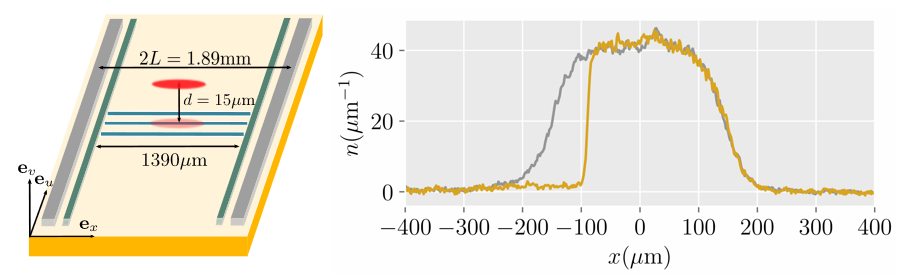
\includegraphics[width=0.90\linewidth]{Atom_chip.png}
%\caption{(a) Schéma de la puce atomique. Les $3$ fils bleus assurent le confinement transverse, les $4$ autres fils (gris) génèrent le potentiel longitudinal. Le nuage atomique, représenté par une ellipse rouge, est piégé à $12~\mu$m au-dessus des fils. (b) Profils de densité linéique extraits par imagerie par absorption. En gris : gaz piégé dans un potentiel quartique. En jaune : après application du faisceau pousseur pendant $30~\mu$s, suivi d’un temps de vol de $1$~ms.}
%\label{fig:setup}
%\end{figure}

%Nous préparons un gaz ultra-froid d’atomes bosoniques de $^{87}$Rb dans l’état $|F=2,m_F=2\rangle$ à l’aide d’un piège magnétique combinant un confinement transverse intense et un confinement longitudinal contrôlé par des courants dans des fils situés à la surface d'une puce atomique. Le système de confinement transverse est réalisé par trois microfils parallèles, parcourus par des courants alternatifs modulés à $400$MHz, qui sont déposés sur la puce (Fig.\ref{fig:setup}(a)). Cette configuration permet non seulement de compenser les effets de rugosité des fils mais aussi de maintenir une indépendance entre les confinements longitudinal et transverse \cite{PhysRevLett.98.263201}.

%Les atomes sont piégés à une distance de $7~\mu$m de la surface de la puce et à $15~\mu$m des microfils, ce qui garantit un confinement transverse très intense. Le potentiel transverse est bien décrit par un potentiel harmonique de fréquence $\omega_{\perp}/2\pi = 2.56$~kHz, et le gaz est refroidi par évaporation par radiofréquence à une température d’environ $T = 100$~nK, pour un potentiel chimique $\mu / k_B = 45$~nK.

%Les rapports $\mu / (\hbar \omega_{\perp}) = 0{,}4$ et $k_B T / (\hbar \omega_{\perp}) = 0{,}8$ placent le gaz dans un régime unidimensionnel. Le couplage effectif en 1D, pour des atomes dans l’état fondamental transverse, est donné par $g = 2 a_{3D} \hbar \omega_{\perp}$, avec $a_{3D} = 5{,}3$~nm la longueur de diffusion tridimensionnelle du $^{87}$Rb \cite{PhysRevLett.89.283202}. Ce régime est caractérisé par un paramètre sans dimension de Lieb $\gamma = m g / (\hbar^2 n_0)$, où $n_0$ est la densité linéique. Les gaz se trouvent profondément dans le régime de quasicondensat, avec une température bien inférieure à la densité $n_0$ \cite{PhysRevLett.91.040403}.

%Stabilité et reproductibilité du piège quartique
%Le piège quartique utilisé dans notre expérience est stabilisé par des courants dans quatre fils placés autour des trois microfils de confinement transverse, permettant de réaliser un piégeage longitudinal avec un potentiel de forme quartique. Ce dispositif assure une densité linéique quasi homogène sur une zone d'environ $250~\mu$m, comme illustré par les profils de densité extraits par imagerie par absorption (Fig.~\ref{fig:setup}(b)). La stabilité et la reproductibilité du piège quartique sont garanties grâce à un contrôle précis des courants, permettant d’ajuster les coefficients du potentiel longitudinal.

%Les paramètres de notre piège longitudinal incluent un champ magnétique homogène $B_0 = 3{,}36$~G et des courants dans les fils de confinement : $I_D = 1.400$~A, $I_{D'} = 1.100$~A, $I_d = 1.090$~A et $I_{d'} = 0.875$~A. Cette configuration permet de réaliser un confinement longitudinal très précis et stable, essentiel pour l'étude de la dynamique des gaz en régime unidimensionnel. La méthode de sélection spatiale, décrite dans \cite{PhysRevLett.133.113402}, permet de réaliser une coupure nette du nuage atomique en éclairant une partie du gaz avec un faisceau lumineux, générant une frontière nette entre les régions de densité nulle et non nulle.

%Paramètres expérimentaux
%Pour réaliser la coupure bipartite, une partie du nuage est illuminée à son extrémité gauche par un faisceau lumineux quasi résonant avec la transition $F=2 \rightarrow F'=3$ de la raie D2. Le faisceau est façonné spatialement à l’aide d’un dispositif à micromiroirs numériques (DMD) et est désaccordé de $15$MHz pour éviter la réabsorption des photons. L’illumination dure $30\mu$s, ce qui permet aux atomes d’acquérir suffisamment d’énergie pour quitter le piège. Ce protocole crée une zone de densité nulle à une extrémité du nuage, comme illustré en jaune sur la Fig.~\ref{fig:setup}(b).

%Une fois la coupure réalisée, le confinement longitudinal est supprimé, mais le confinement transverse est maintenu. Le profil de densité du nuage évolue alors au cours du temps, et cette dynamique est étudiée en enregistrant les profils de densité longitudinale $n(x,t)$ pour différentes durées d’évolution $t$.

%\begin{figure}[!htb]
%\centering
%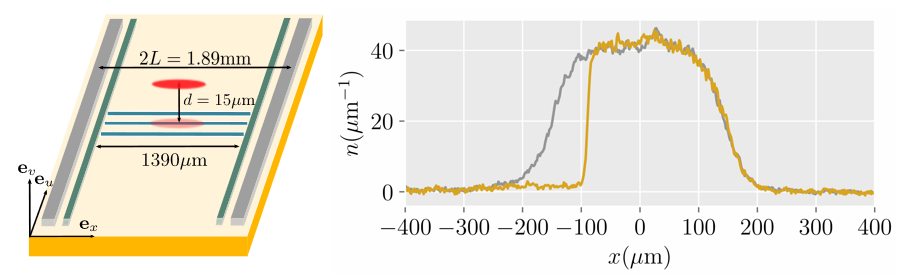
\includegraphics[width=0.90\linewidth]{Atom_chip.png}
%\caption{(a) Schéma de la puce atomique. Les $3$ fils bleus assurent le confinement transverse, les $4$ autres fils (gris) génèrent le potentiel longitudinal. Le nuage atomique, représenté par une ellipse rouge, est piégé à $12~\mu$m au-dessus des fils. (b) Profils de densité linéique extraits par imagerie par absorption. En gris : gaz piégé dans un potentiel quartique. En jaune : après application du faisceau pousseur pendant $30~\mu$s, suivi d’un temps de vol de $1$~ms.}
%\label{fig:setup}
%\end{figure}

\begin{figure}[!htb]
\centering
\includegraphics[width=0.5\linewidth , page = 2 ]{Shemas_2.pdf}
\caption{Schéma à compléter, comprenant plusieurs parties : deux diagrammes temporels montrant l'intensité lumineuse du pulse DMD et de la sonde imageuse, l'intensité des courants de piégeage longitudinal et transverse, un schéma 3D du piège avec un schéma du nuage atomique, un diagramme du DMD similaire à celui de l'article sur la sélection spatiale, un schéma du DMD, ainsi que des schémas 2D représentant l'évolution du nuage à différentes étapes.}
%\label{fig:setup}		
\end{figure}




\subsection{Préparation et Confinement du Gaz Ultra-Froid de $^{87}$Rb}

Nous préparons un gaz ultra-froid d'atomes bosoniques de $^{87}$Rb dans l'état $|F=2,m_F=2\rangle$ à l’aide d'un piège magnétique combinant un confinement transverse intense et un confinement longitudinal contrôlé par des courants dans des fils situés à la surface d'une puce atomique. Le système de confinement transverse est réalisé par trois microfils parallèles déposés sur la puce (Fig.\ref{fig:setup}(a)), parcourus par des courants alternatifs modulés à $400$ MHz. Cette configuration permet de compenser les effets de rugosité des fils et de maintenir une indépendance entre les confinements longitudinal et transverse \cite{PhysRevLett.98.263201}.

Les atomes sont piégés à une distance de $7~\mu$m de la surface de la puce et à $15~\mu$m des microfils, garantissant ainsi un confinement transverse très intense. Le potentiel transverse est bien décrit par un potentiel harmonique de fréquence $\omega_{\perp}/2\pi = 2{,}56$~kHz. Un refroidissement par évaporation par radiofréquence permet d’obtenir un nuage atomique à une température d’environ $T \approx 100$~nK, pour un potentiel chimique $\mu / k_B = 45$~nK.

Les rapports $\mu / (\hbar \omega_{\perp}) = 0{,}4$ et $k_B T / (\hbar \omega_{\perp}) = 0{,}8$ placent le gaz dans un régime unidimensionnel. Le couplage effectif en 1D est donné par $g = 2 a_{3D} \hbar \omega_{\perp}$, avec $a_{3D} = 5{,}3$~nm, la longueur de diffusion tridimensionnelle du $^{87}$Rb \cite{PhysRevLett.89.283202}. Des détails supplémentaires sur l’expérience sont disponibles dans \cite{duboistel-04749900}. Le gaz se trouve profondément dans le régime de quasicondensat, avec un paramètre sans dimension de Lieb $\gamma = m g / (\hbar^2 n_0)$ dans l'intervalle $[0{,}4,0{,}7] \times 10^{-2}$,  tandis que la température satisfait l’inégalité $T \ll n_0^{3/2} \sqrt{\hbar^2 g / m} / k_B$. Ainsi, les gaz obtenus se trouvent profondément dans le régime de quasicondensat \cite{PhysRevLett.91.040403}.

\subsection{Confinement Longitudinal et Stabilisation du Piège Quartique}

Le piégeage longitudinal est assuré par des courants continus circulant dans quatre fils placés de part et d’autre des trois microfils de confinement transverse, comme illustré sur la Fig.\ref{fig:setup}(a). Étant donné que ces fils sont situés loin du centre du nuage atomique, le potentiel longitudinal peut être développé en série polynomiale : $V(x) = \sum_{i=1}^4 a_i x^i$. Les quatre premiers coefficients $a_i$ peuvent être ajustés en modulant les courants dans ces fils. Il est ainsi possible d’annuler les termes linéaire, quadratique et cubique ($a_1 = a_2 = a_3 = 0$), de sorte que le terme dominant du potentiel soit quartique : $V(x) = a_4 x^4$. Une telle forme de potentiel permet d’obtenir une densité atomique quasi homogène sur une région relativement étendue, condition essentielle à l’étude de dynamiques hors équilibre telles que le protocole de coupure bipartite, qui suppose un système semi-infini. Un exemple de profil de densité linéique obtenu dans ce potentiel quartique est représenté en gris sur la Fig.\ref{fig:setup}(b). La densité linéique $n_0$ y reste constante à $10\%$ près sur une distance d’environ $250~\mu$m.

%Le piège longitudinal est réalisé par des courants dans quatre fils placés autour des trois microfils de confinement transverse (Fig.\ref{fig:setup}(a)), permettant de réaliser un potentiel longitudinal de forme quartique. Ce dispositif assure une densité linéique quasi homogène sur une zone d'environ $250\mu$m, comme l'indiquent les profils de densité extraits par imagerie par absorption (Fig.~\ref{fig:setup}(b)).

Les paramètres du piège longitudinal incluent un champ magnétique homogène $B_0 = 3{,}36$~G et des courants dans les fils de confinement : $I_D = 1.400$~A, $I_{D'} = 1.100$~A, $I_d = 1.090$~A, et $I_{d'} = 0.875$~A. Cette configuration permet de garantir un confinement longitudinal très précis et stable, essentiel pour l'étude des dynamiques des gaz en régime unidimensionnel.

\subsection{Sélection Spatiale et Réalisation de la Coupure Bipartite}

Pour réaliser expérimentalement une bipartition initiale nette, nous utilisons la méthode de sélection spatiale introduite dans \cite{PhysRevLett.133.113402}. Une partie du nuage, initialement dans un état stationnaire global dans le piège quartique, est illuminée à son extrémité gauche par un faisceau lumineux quasi résonant avec la transition $F=2 \rightarrow F'=3$ de la raie D2, se propageant perpendiculairement à l’axe $x$. Les atomes exposés subissent une pression de radiation : après $30~\mu$s d’illumination, correspondant à environ 15 cycles absorption/réémission, ces atomes acquièrent une énergie suffisante pour quitter le piège. Le faisceau est façonné spatialement à l’aide d’un dispositif à micromiroirs numériques (DMD) afin de ne cibler qu’un bord du gaz. Ce protocole produit une frontière nette entre une région vide et un gaz quasi homogène, rendue possible par l’utilisation du piège quartique. La résolution de cette coupure est limitée principalement par la résolution du système d’imagerie (quelques microns). L’éventuelle réabsorption des photons diffusés par les atomes non illuminés est réduite en désaccordant le faisceau pousseur de $15$MHz par rapport à la transition D2. Un exemple de profil de densité après application de ce protocole est illustré en jaune sur la Fig.\ref{fig:setup}(b).

%Pour réaliser une coupure bipartite nette, une partie du nuage est illuminée à son extrémité gauche par un faisceau lumineux quasi résonant avec la transition $F=2 \rightarrow F'=3$ de la raie D2. Le faisceau est façonné spatialement à l’aide d’un dispositif à micromiroirs numériques (DMD) et désaccordé de $15$ MHz pour éviter la réabsorption des photons. L’illumination dure $30~\mu$s, ce qui permet aux atomes d’acquérir suffisamment d’énergie pour quitter le piège. Ce protocole génère une frontière nette entre les régions de densité nulle et non nulle, créant ainsi une zone de densité nulle à une extrémité du nuage (Fig.~\ref{fig:setup}(b)).

\subsection{Dynamique Après Coupure}
Une fois la coupure réalisée, le confinement longitudinal est supprimé, mais le confinement transverse est maintenu. La frontière initialement abrupte s’élargit au cours du temps. Cette dynamique est étudiée en enregistrant les profils de densité longitudinale $n(x;t)$ pour différentes durées d’évolution $t$.

\begin{figure}[!htb]
\centering
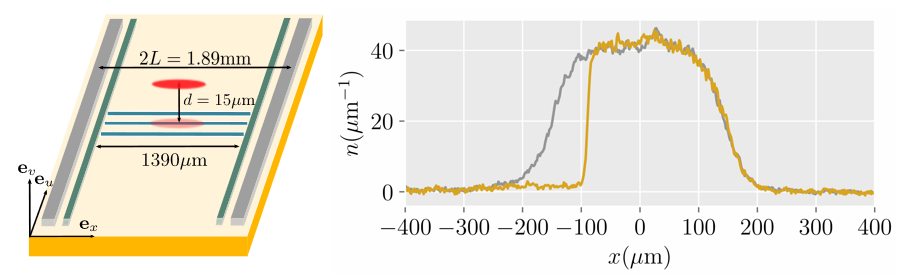
\includegraphics[width=0.90\linewidth]{Atom_chip.png}
\caption{(a) Schéma de la puce atomique. Les $3$ fils bleus assurent le confinement transverse, les $4$ autres fils (gris) génèrent le potentiel longitudinal. Le nuage atomique, représenté par une ellipse rouge, est piégé à $12~\mu$m au-dessus des fils. (b) Profils de densité linéique extraits par imagerie par absorption. En gris : gaz piégé dans un potentiel quartique. En jaune : après application du faisceau pousseur pendant $30~\mu$s, suivi d’un temps de vol de $1$~ms.}
\label{fig:setup}
\end{figure}





\section{Prédictions de la GHD}\label{sec.GHDpredictions}
\label{sec:ghd}

Le dispositif expérimental décrit ci-dessus peut être analysé théoriquement comme suit. Au cours de l'évolution temporelle, la frontière nette initiale du nuage devient plus lisse et les dérivées temporelles des quantités locales diminuent. Après un certain temps, après un lissage, on s'attend à ce que le gaz puisse être décrit localement par des états stationnaires.

Les états stationnaires du modèle de Lieb-Liniger sont complètement caractérisés par leur distribution de rapidité $\rho(\theta)$. Alternativement, ces états peuvent être caractérisés par le facteur d'occupation $\nu(\theta)$.% qui prend des valeurs entre 0 et 1, et qui est liée à la distribution de rapidité $\rho(\theta)$ par
%\begin{equation}
%\nu(\theta) = \frac{\rho(\theta)}{\rho_s(\theta)} \mbox{, \qquad où \qquad } \rho_s(\theta) =
%\frac{m}{2\pi \hbar} + \int \frac{d\theta'}{2\pi} \Delta(\theta-\theta') \rho(\theta') ,
%\end{equation}
%et $\Delta(\Theta) = \frac{2g}{\left(\frac{g^2}{\hbar} + \hbar \Theta^2\right)}$ est le "décalage de diffusion" dans le modèle de Lieb-Liniger. Les fonctions $\nu$ et $\rho$ sont en correspondance biunivoque, et dans ce qui suit, nous utilisons alternativement $\rho$ ou $\nu$. [Pour une introduction à ce formalisme, nous nous référons aux notes de cours \cite{doyon2020lecture} ou à la Section 1 de l'article de revue \cite{bouchoule_generalized_2022}.]

Puisque nous supposons une stationnarité locale, le système dans son ensemble est décrit par une distribution de rapidité dépendante du temps et de la position $\rho(x,\theta ; t )$, ou équivalemment par le facteur d'occupation dépendant du temps et de la position $\nu(x,\theta ; t)$. Ce dernier conduit à des calculs plus simples, tandis que le premier est particulièrement utile pour extraire la densité linéaire, qui est donnée par
\begin{equation}
    \label{eq:lineardensity}
	n(x;t) = \int d\theta \, \rho(x,\theta ; t ) .
\end{equation}

Les équations de GHD \cite{bertini_transport_2016,castro-alvaredo_emergent_2016} prédisent l'évolution temporelle de $\rho(x,\theta ; t)$, ou équivalemment de $\nu(x,\theta ; t)$. Lorsqu'elles sont écrites en termes du facteur d'occupation $\nu(x,\theta ; t )$, les équations de GHD prennent la forme d'une équation convective :
%\begin{subequations}
%\label{eq:GHD}
\begin{equation}
\label{eq:nu.cont}
\frac{\partial \nu}{\partial t} + v^{\rm{eff}}_{[\nu]} \frac{\partial \nu}{\partial x} = 0 ,
\end{equation}
et une deuxième relation qui fixe la vitesse effective $v^{\rm{eff}}_{[\nu]}$ comme une fonctionnelle de la distribution locale de rapidité (cf {??}).
%\begin{equation}
%v_{[\nu]}^{\rm{eff}}(\theta) = \theta - \int \Delta(\theta-\theta') \left( v^{\rm{eff}}_{[\nu]}(\theta) - v^{\rm{eff}}_{[\nu]}(\theta') \right) \rho(\theta') d\theta' .
%\end{equation}
%\end{subequations}
%Plus précisément, l'équation~(\ref{eq:GHD}a) est la forme à l'échelle d'Euler de la GHD, une équation sans diffusion valable aux grandes échelles. Des corrections diffuses, qui apparaissent sous forme d'un terme de type Navier-Stokes~\cite{de2018hydrodynamic,de2019diffusion,bastianello2020thermalization,de2022correlation}, ou même des corrections dispersives~\cite{de2023hydrodynamic}, ont également été étudiées théoriquement. Cependant, ces effets sont secondaires et n'ont pas été observés expérimentalement jusqu'à présent. Nous verrons plus bas que nos données expérimentales respectent le collage d'échelle attendu à l'échelle d'Euler (Fig.~\ref{fig:euler}), de sorte que ces effets semblent négligeables dans notre situation, du moins pour l'analyse des profils de frontière. Cela est également compatible avec une étude théorique récente dans le régime de faible interaction, qui a conclu que les effets diffusiques devraient être très faibles~\cite{moller2024identifying}. Par conséquent, dans cet article, nous ignorons la possibilité d'effets diffusiques secondaires (ainsi que tous les effets d'ordre supérieur) dans notre modélisation et nous nous en tenons à l'équation de GHD à l'échelle d'Euler ci-dessus.
\begin{figure}[!htb]
	\centering
	\includegraphics[width=\textwidth , page = 5 ]{Shema.pdf}
	\caption{
(a) À l'instant $t = 0^+$, immédiatement après le « quench bipartite » en $x = 0$, le facteur d'occupation est donné par $\nu(x, \theta ; t = 0^+) = \nu_0(\theta)$ pour $x > 0$ et est nul pour $x < 0$. Le bord initial représenté en tirets par l'ensemble des points $(x(s; t = 0^+) = 0,\ \theta(s; t = 0^+))$.
(b) Densité spatiale linéique $n(x)$ : en pointillés, $n(x; t = 0^-) = \int \rho(x, \theta; t = 0^-) \, \mathrm{d}\theta = n_0 = 56~\mu\mathrm{m}^{-1}$ juste avant le quench ; en ligne pleine, $n(x; t = 0^+) = n_0$ pour $x > 0$ et $0$ pour $x < 0$.
(c) À gauche de la coupure ($x < 0$) : en pointillés, $\nu(x, \theta ; t = 0^-) = \nu_0(\theta)$ ; en ligne pleine, $\nu(x, \theta ; t = 0^+) = 0$.
(d) À droite de la coupure ($x > 0$), le facteur d'occupation reste inchangé : $\nu(x, \theta ; t = 0^+) = \nu_0(\theta)$.
(e) À l'instant $t = 18~\mathrm{ms}$, après l'évolution balistique post-quench, le facteur d'occupation est donné par $\nu^\ast(x(s;t)/t, \theta) = \nu_0(\theta)$ pour $\theta < \theta(s;t)$, et nul pour $\theta > \theta(s;t)$, résolvant l'équation~(\ref{eq:nuetoile}), pour $t>0$. $\nu(x(s;t), \theta(s;t))(=\nu^\ast(x(s;t)/t, \theta(s;t)))$ est invarient de la déformation ie de $t>0$.  Le bord représenté en tirets par l'ensemble des points $(x(s; t)/t,\, \theta(s; t))$. Étant donné que la coupure initiale est en $x = 0$ et que l’évolution du bord est balistique, cette courbe résoud $v^{\mbox{\tiny eff}}_{[\nu^\ast(x(s; t)/t, \cdot) ]}(\theta(s; t)) = x(s; t)/t = v(s)$ (\ref{eq:nu.cont}).
(f) Densité spatiale réduite $n^\ast(x/t; t)$.
(g) Pour les atomes à droite de la coupure : en pointillés, $\nu^\ast(x(s;t)/t, \theta) = \nu_0(\theta)$ ; en ligne pleine, $\nu^\ast(x(s;t)/t, \theta) = \nu_0(\theta)$ pour $\theta < \theta(s;t)$ et nul pour $\theta > \theta(s;t)$. Le raisonnement est similaire pour les atomes à gauche de la coupure.
}
	\label{fig:BiPart.coupure1}
	
\end{figure}

%\begin{figure}[hbt]
%    \centering
    %\includegraphics[width=0.7\textwidth]{Figures/figure_nustar.pdf}
%    \caption{Facteur d'occupation $\nu^* (v,\theta)$ résolvant l'équation (\ref{eq:nuetoile}) pour un ratio d'occupation initial $\nu_0 (\theta)$ dans la moitié droite du système correspondant à un équilibre thermique à température $T$. La ligne verte pointillée est la courbe $\theta^*(v)$, c'est-à-dire l'ensemble des points $(v,\theta)$ tels que $v^{\rm eff}_{[\nu^* (v,\cdot)]} (\theta) = v$. [Paramètres : 
%    $\gamma_0=mg/(n_0\hbar^2)=0.005$, $k_B T \hbar^2/(mg^2) = 365$, proches des paramètres expérimentaux des jeux de données ci-dessous.]}
%    \label{fig:nu_star}
%\end{figure}

Pour une bipartition initiale dont la discontinuité est située à $x=0$, la solution de \eqref{eq:GHD} est invariante le long des rayons de vitesse constante $x/t$~\cite{bertini_transport_2016,castro-alvaredo_emergent_2016}. En d'autres termes, l'équation \eqref{eq:GHD} implique que, pour cette classe d'états initiaux, la distribution du facteur d'occupation local et donc toutes les propriétés locales du gaz, dépendent de $x$ et $t$ uniquement à travers la quantité $v=x/t$. La solution de l'équation \eqref{eq:GHD} peut donc être écrite en utilisant le facteur d'occupation le long des rayons $\nu^*(v,\theta)$ tel que
\begin{equation}
	\label{eq:nuvsnuetoile}
    \nu(x,t,\theta) = \nu^*( x/t,\theta).
\end{equation}

Pour la situation considérée dans cet article, où initialement un état de vide est situé pour $x < 0$ et un état de distribution du facteur d'occupation $\nu_0$ pour $x > 0$, la solution $\nu^*(v,\theta)$ est paramétrée par une rapidité de bord $\theta^*$ selon~\cite{bertini_transport_2016,castro-alvaredo_emergent_2016}
\begin{equation}
	\label{eq:nuetoile}
    \nu^*(v,\theta) = \left\{
    	\begin{array}{ccc}
    		\nu_0(\theta) & \text{si} & \theta < \theta^* \\
    		0 & \text{si} & \theta > \theta^* \\
   		\end{array}
    	\right. \quad \text{où} \quad  v^{\rm{eff}}_{[\nu^*(v,.)]}(\theta^*) = v.
\end{equation}
Cette équation peut être résolue numériquement pour toute distribution initiale donnée $\nu_0(\theta)$, voir la Fig.~\ref{fig:BiPart.coupure1} pour un exemple. Avec l'équation~\eqref{eq:nuvsnuetoile}, elle décrit entièrement le système à l'échelle d'Euler. Notez que, pour calculer la densité linéaire $n(x,t)$ afin de comparer avec les profils de densité expérimentaux, on utilise l'équation (\ref{eq:lineardensity}).

%\paragraph{Solution pour un système initialement dans l'état fondamental.}
%Pour illustrer le formalisme ci-dessus, explorons ses implications pour le cas spécial où la moitié droite du système est initialement dans l'état fondamental. Dans ce cas, le facteur d'occupation initial $\nu_0 (\theta)$ est une mer de Fermi : $\nu_0(\theta) = 1$ pour $|\theta| < \Delta\theta_0$, et $\nu_0(\theta) = 0$ sinon. Le rayon de Fermi $\Delta\theta_0$ dépend de la densité linéaire du gaz dans cette région, qui est constante. La distribution du facteur d'occupation se découpe ainsi en deux régions : pour $|\theta| > \Delta\theta_0$, $\nu_0(\theta) = 0$, et pour $|\theta| < \Delta\theta_0$, $\nu_0(\theta) = 1$. Au temps $t=0$, nous avons donc une discontinuité dans la distribution du facteur d'occupation à $\theta=\pm \Delta\theta_0$.

\section{Données expérimentales}\label{sec.ed}

L’état initial est préparé selon le protocole décrit en section~\ref{sub_pisih}. Le confinement longitudinal est ensuite supprimé, tandis que le confinement transverse est maintenu, afin d'étudier la dynamique le long de l’axe longitudinal.

Les profils de densité en bord obtenus pour des temps d’évolution compris entre $\tau = 10$~ms et $\tau = 18$ms sont présentés en Fig.\ref{fig:euler}(a), en fonction de la variable réduite $v = x/\tau$. L’excellent recouvrement des différents profils indique que l’échelle d’Euler est atteinte dans cet intervalle temporel. Au-delà de $\tau = 18$~ms, la dynamique longitudinale ne peut plus être explorée expérimentalement, en raison de la taille finie du gaz initial, préparé dans une configuration semi-homogène.

Pour des temps d’évolution plus courts, les profils de bord mesurés présentent une forme plus lissée que celle prédite par les équations de GHD à l’échelle d’Euler. Cette différence peut s’expliquer soit par une invalidité de l’approximation d’Euler dans ce régime transitoire, en lien avec de fortes variations de densité, soit par le fait que la coupure initiale à $t = 0$ n’est pas parfaitement abrupte, ce qui confère au bord initial une largeur finie.

\begin{figure}[!htb]
\centering
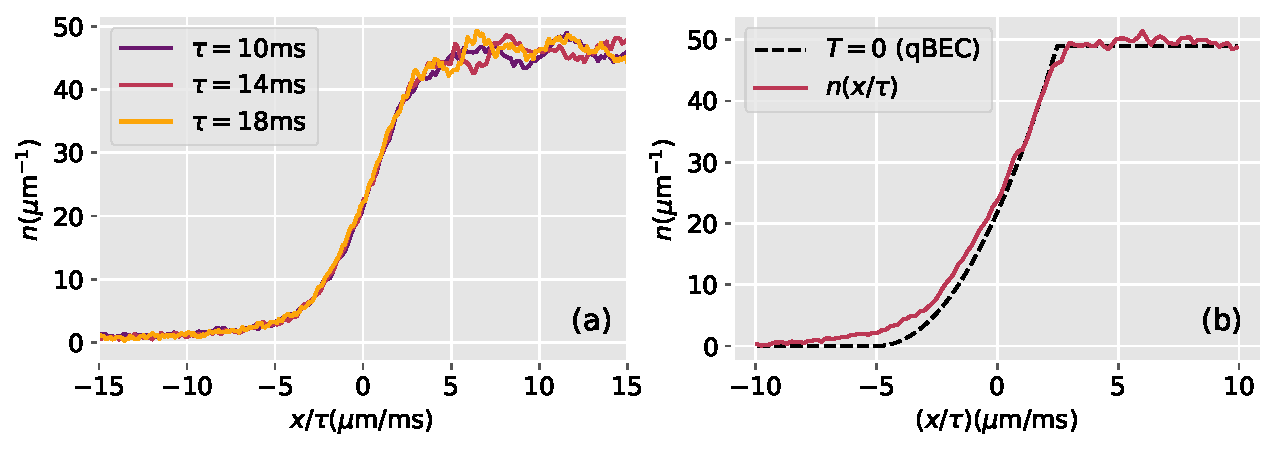
\includegraphics[width=1.0\linewidth]{DWD_GPE_vs_exp_V2.pdf}
\caption{(a) Profils de densité aux bords obtenus pour différents temps d’évolution $\tau$, représentés en fonction de $x/\tau$ ; (b) Comparaison du profil de bord mesuré avec la prédiction à température nulle issue de la GHD dans le régime quasi-condensat, donnée par l’équation~\eqref{eq:GPE}. Cette dernière constitue une excellente approximation pour la valeur du paramètre d’interaction correspondant aux données, soit $\gamma = 4{,}6 \times 10^{-3}$ (voir Fig.\ref{fig:boundary_profiles_theory}). Le profil de bord présenté en (b) est obtenu après un temps d’expansion de 10ms et provient d’un jeu de données différent de celui de la figure (a).}
\label{fig:euler}
\end{figure}

La figure~\ref{fig:euler}(b) présente une comparaison entre le profil de bord mesuré $n(v)$ et la prédiction théorique fondée sur un état initial à température nulle, supposé être l’état fondamental. Pour la valeur du paramètre de Lieb $\gamma = 4{,}6 \times 10^{-3}$, le profil est pratiquement indiscernable de celui obtenu dans le régime de quasi-condensat, justifiant l’utilisation de l’équation~\eqref{eq:GPE} pour la comparaison.

L’accord entre la prédiction théorique et les données expérimentales est satisfaisant, en particulier dans la région de forte densité. Les écarts observés par rapport à la forme parabolique prédite peuvent être attribués à des effets liés à une entropie non nulle, qui seront analysés dans la section suivante.

\section{Sonder la distribution locale des rapidités}
\label{sec:local}

Pour un état initial du gaz correspondant à un facteur d'occupation lisse $\nu(\theta)$ (par exemple un état thermique), le facteur d'occupation $\nu^*(x/t,\theta)$ à rapport $x/t$ fixé est attendu comme étant fortement asymétrique en fonction de $\theta$, selon l'équation~\eqref{eq:nuetoile}. En effet, du côté droite, il présente une discontinuité du type saut, similaire à celle du facteur d'occupation de l’état fondamental, tandis que du côté gauche, il reste lisse. Afin de révéler ces caractéristiques particulières de l’état local du gaz, nous utilisons le protocole introduit dans la Réf.~\cite{dubois_probing_2024} pour sonder la distribution locale des rapidités, comme expliqué ci-après.

Nous laissons d’abord le gaz se dilater pendant un temps $t=18~\mathrm{ms}$, de sorte que le bord s’étale sur une large zone d’environ $350~\mathrm{\mu m}$, comme illustré en Fig.~\ref{fig:BiPart.coupure1} (e)-(f) et  Fig ~\ref{fig:simul_deformation} (a).  
Nous sélectionnons ensuite une tranche du gaz comprise dans l’intervalle $[x_0-\ell/2, x_0+\ell/2]$, en éliminant tous les atomes situés hors de cette tranche à l’aide d’un faisceau de poussée~\cite{dubois_probing_2024}(Fig \ref{fig:BiPart.coupure2} (a)--(c)). 

\begin{figure}[!htb]
	\centering
	\includegraphics[width=\textwidth , page = 6 ]{Shema.pdf}
	\caption{
(a) À l'instant $\tau = 0^+$, immédiatement après la sélection de la tranche centrée en $x = x_0$ et de largeur $\ell$, la distribution de rapidité localement résolue est donnée par $\rho(x,\theta ; \tau = 0^+) = \nu(x, \theta ; t = 18~\mathrm{ms}) \, \rho_s(x,\theta ; t = 18~\mathrm{ms})$ pour $\vert x - x_0 \vert < \ell/2$, et est nulle pour $\vert x - x_0 \vert > \ell/2$. Le bord gauche immédiatement après la sélection est représenté en pointillés par l’ensemble des points $(x_g(s; \tau = 0^+),\ \theta_g(s; \tau = 0^+))$, et le bord droit en tiret-point par l’ensemble des points $(x_d(s; \tau = 0^+),\ \theta_d(s; \tau = 0^+))$. Le bord complet est donc la concaténation de ces deux ensembles. 
(b) Densité linéique spatiale $n(x)$ : en pointillés, $n(x; t = 18~\mathrm{ms})$ juste avant la sélection ; en ligne pleine, $n(x; \tau = 0^+)$, égal à $n(x; t = 18~\mathrm{ms})$ pour $\vert x - x_0 \vert < \ell/2$ et nul ailleurs. 
(c) Distribution de rapidité après sélection, $\Pi(\theta) = \int \rho(x,\theta ; \tau)\,\mathrm{d}x$, invariante sous l’évolution unidimensionnelle, représentée en rouge. La distribution localement résolue en $x(s; \tau = 0^+)$, $\rho(x(s; \tau = 0^+), \theta ; \tau = 0^+)$, est représentée en pointillés. Cette distribution est localement conservée, i.e., $\rho(x(s; \tau), \theta(s; \tau))$ reste inchangée au cours de l’évolution unidimensionnelle, indépendamment de $\tau$. 
(e) Distribution localement résolue $\rho(x, \theta ; \tau = 30~\mathrm{ms})$ après une évolution unidimensionnelle de $30~\mathrm{ms}$. Le bord gauche est représenté en pointillés par les points $(x_g(s; \tau = 30~\mathrm{ms}),\ \theta(s; \tau = 30~\mathrm{ms}))$, et le bord droit en tiret-point par $(x_d(s; \tau = 30~\mathrm{ms}),\ \theta(s; \tau = 30~\mathrm{ms}))$. 
(f) Densité spatiale réduite $n(x; \tau = 30~\mathrm{ms})$. 
(g) Distribution de rapidité $\Pi(\theta)$ après la sélection (identique à celle de (c)).
}
	\label{fig:BiPart.coupure2}
	
\end{figure}
 
En Fig.~\ref{fig:simul_deformation}(a), nous présentons le profil de densité mesuré $1$ ms après la sélection de la tranche.  
L’ajustement à une fonction rectangulaire lissée donne $x_0 = 18\,\mu$m.  
Pour les calculs, la largeur $\ell$ sera déterminée à partir du nombre d’atomes sélectionnés (voir ci-dessous).  
Enfin, nous laissons cette tranche se dilater en 1D pendant un temps d’expansion $\tau$, puis nous mesurons la densité longitudinale $\tilde{n}(x,\tau)$.  
Celle-ci reflète la distribution totale des rapidités dans la tranche $\Pi(\theta) = \int \rho(x, \theta ; \tau > 0)\, dx = \int_{x_0 - \ell/2}^{x_0 + \ell/2} \rho(x, \theta ; \tau = 0^+)\, dx$, car pour $\tau \rightarrow \infty$, on s’attend à ce que $\tau \tilde{n}( \tau * \theta - x_0  ;\tau) \simeq \Pi(\theta)$.  
L’asymétrie attendue de $\Pi$ devrait ainsi induire une asymétrie de la densité $\tilde{n}(x,\tau)$ en fonction de $x$.  
Nous observons effectivement cette asymétrie dans nos profils d’expansion, comme illustré en Fig.~\ref{fig:simul_deformation}(b) pour un temps d’expansion $\tau=30$ ms.

\begin{figure}[!htb]
\centering
\begin{tikzpicture}
    \node[rectangle, draw = none] (bord) at (0,0) {
        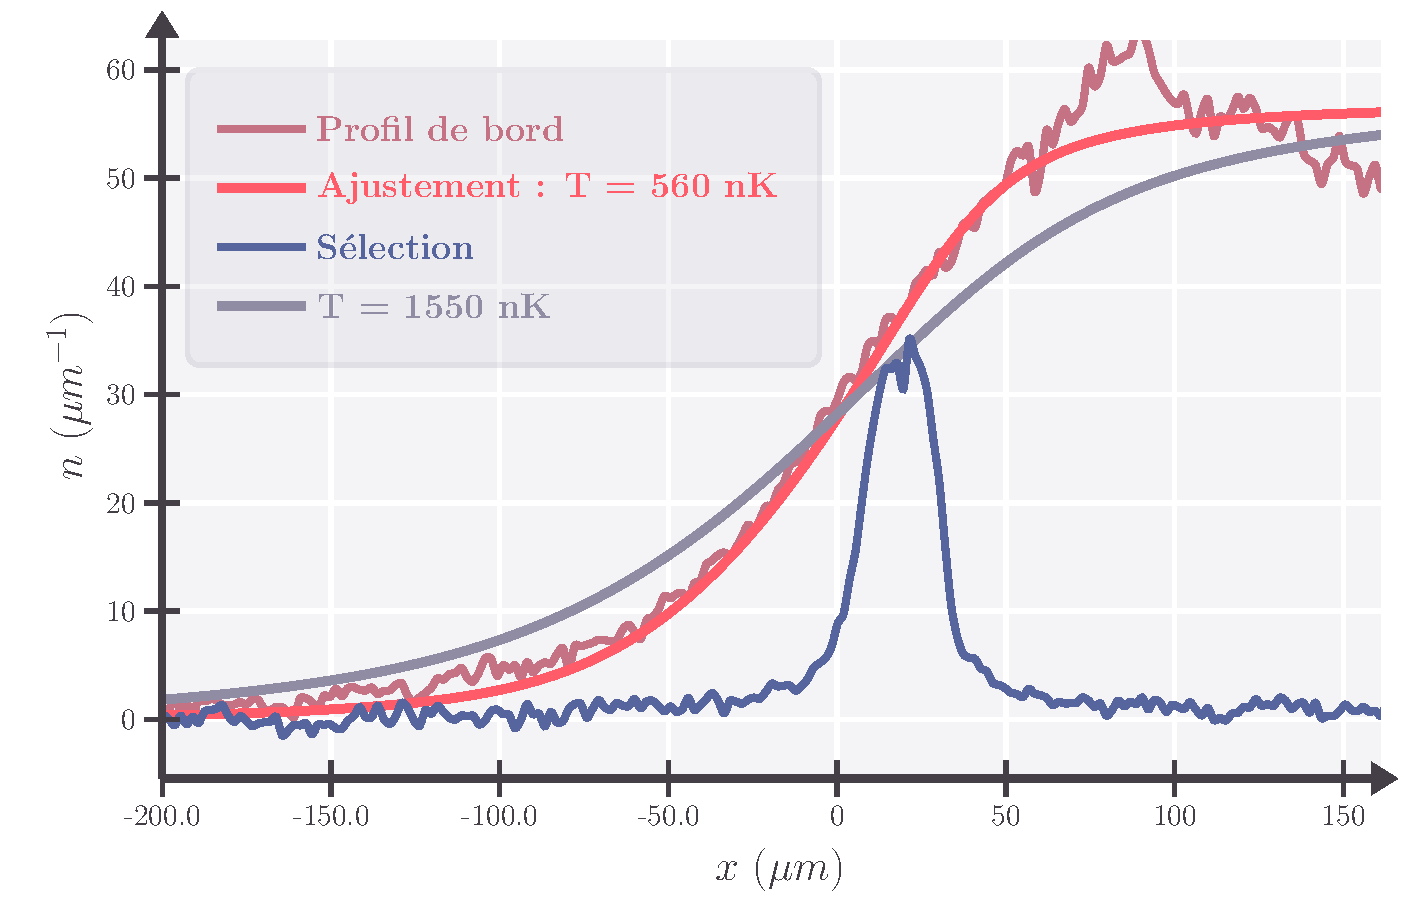
\includegraphics[width=0.5\textwidth , page = 1]{Figures}
    };
    \node[circle, draw=none, above=0cm of bord , shift={( -2.5cm , -0.5cm )} ] {(a)};
    
    \node[right=1mm of bord , shift={( -0.5cm , 0cm )}] (assy) {
        \includegraphics[width=0.5\textwidth , page = 2 ]{Figures}
    };
    \node[circle, draw=none, above=0cm of assy , shift={( -2.5cm , -0.5cm )}] {(b)};
\end{tikzpicture}
\caption{(a) {\it Profil de bord et tranche sélectionnée.} Le profil de bord après $18\,\mathrm{ms}$ est montré en rouge. L'ajustement thermique donne une température $T = 560\,\mathrm{nK}$ (orange). Le profil de densité mesuré $1\,\mathrm{ms}$ après la sélection de la tranche est en bleu. (b) {\it Asymétrie du profil d’expansion de la tranche.} Le profil de densité après une expansion pendant $\tau = 30\,\mathrm{ms}$ est comparé à son image miroir. Le centre de symétrie $x_s = -17\,\mu$m minimise la distance quadratique $\delta^2 = \int dx\, (\tilde{n}(x) - \tilde{n}(2x_s - x))^2$.}
\label{fig:simul_deformation}
\end{figure}

Pour aller au-delà de cette observation qualitative, nous effectuons un calcul GHD à l’échelle d’Euler du profil d’expansion, en supposant que l’état initial est thermique.  
La température est obtenue par ajustement du profil de bord avant la sélection de la tranche, comme indiqué en Fig.~\ref{fig:simul_deformation}(a), ce qui donne $T = 560$ nK.  
Le potentiel chimique est ajusté afin que la densité linéaire initiale corresponde à celle mesurée dans la région $x > 0$, avant l’élargissement du bord.  
À partir du profil initial, nous simulons à la fois l’élargissement du bord et l’expansion de la tranche en GHD, en supposant une découpe parfaite, c’est-à-dire $\nu(x,\theta) = 0$ pour $|x - x_0| > \ell/2$ et $\nu(x,\theta)$ inchangé sinon.  
La largeur $\ell$ est ajustée de sorte que le nombre d’atomes sélectionnés dans la simulation corresponde à celui mesuré expérimentalement après expansion, et on obtient $\ell = 24\,\mu$m.  

Le profil d’expansion simulé est montré en Fig.~\ref{fig:simul_expansion}(a).  
Il présente une forte asymétrie, comme attendu, avec un bord droit abrupt et une densité nulle au-delà d’un certain point.  
Cependant, cette chute est moins marquée que celle prédite pour la distribution locale des rapidités $\rho(x_0,\theta)$ à $x = x_0$. Deux effets contribuent à cet élargissement :  
(i) la distribution en rapidité n’est pas homogène à l’intérieur de la tranche, si bien que $\Pi(\theta)$ diffère de $\ell \rho(x_0,\theta)$, comme le montre la comparaison entre la ligne marron pleine et la ligne pointillée en Fig.~\ref{fig:simul_expansion}(a) ;  
(ii) le temps d’expansion est fini, de sorte que le profil observé $\tilde{n}(x, {\tau} )$ ne correspond pas exactement à $\Pi((x-x_0)/\tau)/\tau$, comme le montre la comparaison entre les courbes marron et rouge.



%l'ensemble $\{(x_g(1; \tau = 0^+) ,\ \theta(1; \tau = 0^+)) , \cdots , (x_g(q; \tau = 0^+) ,\ \theta(q; \tau = 0^+)) , (x_d(1; \tau = 0^+) ,\ \theta(1; \tau = 0^+)) , \cdots , (x_d(q; \tau = 0^+) ,\ \theta(q; \tau = 0^+)) \}$ ou $q$ est la taille des deux ensemble.



\begin{figure}[!htb]
\centering
\begin{tikzpicture}
    \node[rectangle, draw = none] (exp) at (0,0) {
       \includegraphics[width=0.5\textwidth , page = 3]{Figures}
    };
    \node[circle, draw=none, above=0cm of exp , shift={( -2.5cm , -0.5cm )} ] {(a)};
    
    \node[right=1mm of exp , shift={( -0.5cm , 0cm )}] (pi) {
       \includegraphics[width=0.5\textwidth , page = 4]{Figures}
    };
    \node[circle, draw=none, above=0cm of pi , shift={( -2.5cm , -0.5cm )}] {(b)};
\end{tikzpicture}
\caption{(a) {\it Profil de densité après expansion de la tranche : effets de la largeur finie et du temps d’expansion fini.} Courbe orange : profil obtenu par simulation GHD après expansion pendant $\tau = 30$ ms, avec $T = 560$ nK. Courbe marron : distribution asymptotique $\Pi((x - x_0)/\tau)/\tau$. Courbe pointillée noire : approximation $\ell \rho(x_0, (x - x_0)/\tau)/\tau$ dans le cas d’une tranche étroite. (b) {\it Comparaison aux données expérimentales.} En bleu : profil expérimental après expansion pendant $\tau = 30$ ms. En orange : simulation GHD avec $T = 560$ nK. En magenta : ajustement du profil expérimental donnant $T = 1550$ nK.}
\label{fig:simul_expansion}
\end{figure}

Nous comparons ensuite le profil d'expansion simulé par la GHD avec les données expérimentales. Comme montré en Fig.~\ref{fig:simul_expansion}(b), le profil prédit reproduit les principales caractéristiques du profil d'expansion observé expérimentalement. Des écarts atteignant 25\,\% sont cependant visibles dans la partie centrale du profil. Afin d'obtenir un meilleur accord entre données et calculs, nous avons ajusté le profil d'expansion expérimental avec le calcul GHD en utilisant la température de l'état initial comme paramètre d'ajustement. Le résultat, représenté par la ligne magenta dans la Fig.~\ref{fig:simul_expansion}(b), donne une température $T=1550$~nK, plus de deux fois supérieure à celle obtenue en ajustant le profil au bord. Le profil au bord calculé pour cette température n'est pas compatible avec le profil expérimental, comme le montre la Fig.~\ref{fig:simul_expansion}(b).

Une des raisons de l'échec de nos tentatives de reproduction du profil de densité après l'expansion de la tranche réside dans la présence de queues à droite du profil expérimental — voir le profil de densité dans la Fig.~\ref{fig:simul_expansion}(b). Ces queues sont absentes des calculs GHD à l’échelle d’Euler car la fonction d’occupation dans la tranche s’annule strictement au-delà d’une certaine rapidité. L’origine de ces queues reste incertaine. Elles pourraient être dues à des effets de bord associés à la procédure de sélection de tranche, les atomes en bordure étant chauffés par le faisceau de poussée. Il est également possible qu’un effet diffusif, non pris en compte dans la GHD à l’échelle d’Euler, intervienne au début de la déformation du bord, lorsque les gradients sont importants.

\section{Détails sur les calculs}
\label{sec:calcule}

On fait l'hypothèse que le système est dans un état thermique. Cela implique que la fonction $w$ qui paramétrise l'opérateur charge (cf. ??) vérifie :

\begin{eqnarray*}
	w(\theta) & = &  \beta(\varepsilon(\theta) - \mu),
\end{eqnarray*}

avec $\beta = (k_B T)^{-1}$ et $\varepsilon(\theta) = \frac{m \theta^2}{2}$. On peut réécrire cette relation en minimisant l'entropie de Yang-Yang (cf. ??) et en injectant la forme du facteur d'occupation $\nu = \rho/\rho_s = (1+e^{\beta \epsilon})^{-1}$ . On obtient alors une équation de type point fixe :

\begin{eqnarray*}
	\beta \epsilon & = & \beta \epsilon_0 -  \frac{\Delta}{2\pi} \star \ln \left( 1 + e^{-\beta \epsilon} \right) ,
\end{eqnarray*}

avec $\epsilon_0 = \varepsilon - \mu$. Cette équation est bien définie et converge (cf. ??). Pour s'en convaincre, on peut calculer la norme du déterminant du jacobien de l'application. Si elle est inférieure à 1, on est assuré de la convergence. 

L'équation étant non linéaire, pour garantir la convergence vers la bonne solution (évitant les cycles), on itère la suite suivante :

\begin{eqnarray*}
	\beta \epsilon_{n+1} & = & \beta \epsilon_0 -   \frac{\Delta}{2\pi} \star \ln \left( 1 + e^{-\beta \epsilon_n} \right) ,
\end{eqnarray*}

jusqu'à ce que la distance entre deux itérations successives soit suffisamment petite : ici $\beta \Vert \epsilon_{n+1} - \epsilon_n \Vert < 10^{-12}$.

Ainsi, en fixant le couple $(\mu, T)$, on obtient $\epsilon$, puis $\nu$, puis enfin $\rho_s$ via :

\begin{eqnarray*}
	2\pi \rho_s & = & \frac{m}{\hbar} \ast 1^{\mathrm{dr}},
\end{eqnarray*}

où la fonction "habillée" $f^{\mathrm{dr}}$ est définie par :

\begin{eqnarray*}
	f^{\mathrm{dr}} & = & f + \frac{\Delta}{2\pi} \star ( \nu \ast f^{\mathrm{dr}} ),
\end{eqnarray*}

ce qui est une équation linéaire. Numériquement, on la résout sous la forme :

\begin{eqnarray*}
	\left\{ \mathrm{id} - \frac{\Delta}{2\pi} \star ( \nu \ast \cdot ) \right\} f^{\mathrm{dr}} & = & f.
\end{eqnarray*}

La densité physique est alors obtenue par $\rho = \nu \ast \rho_s$. Expérimentalement, on mesure la densité homogène $n_0 = 56~\mathrm{\mu m^{-1}}$ (voir Fig. \ref{fig:BiPart.insitut}). À température fixée, on ajuste donc le potentiel chimique $\mu$ pour satisfaire la contrainte :

\begin{eqnarray*}
	n_0 & = & \int \rho(\theta) \, d\theta.
\end{eqnarray*}

L'équation (\ref{eq:nuetoile}) implique :

\begin{eqnarray*}
	\nu(x(s;t), \theta(s;t)) & = & \nu(x(s;0), \theta(s;0)),
\end{eqnarray*}

ce qui signifie que $\nu$ est constant au cours du temps si on suit le couple $(x(s;t), \theta(s;t))$ — c’est la vision lagrangienne en hydrodynamique. La graduation fixe des axes donne la vision eulérienne. Cela implique également :

\begin{eqnarray*}
	\partial_t \left( \begin{array}{c} x(s;t) \\ \theta(s;t) \end{array} \right) & = & \left( \begin{array}{c} v^{\mathrm{eff}}_{[\nu]}(\theta(s;t)) \\ 0 \end{array} \right),
\end{eqnarray*}

d’où $\theta(s;t) = \theta(s;0) \equiv \theta(s)$. On note $\Gamma_t \doteq \{(x(s;t), \theta(s;t))\}$. À l’intérieur de ce contour, le facteur d’occupation est indépendant de $x$ (voir Fig. ??), donc il est conservé au cours du temps :

\begin{eqnarray*}
	\nu(x(s,t), \theta(s)) & = & \nu_0(\theta),
\end{eqnarray*}

ce qui est le cas dans tout le protocole. On peut ainsi calculer l’évolution du contour au cours du temps.


\subsection{Simulation de la déformation du bord} 

Dans la partie "déformation du bord" (Fig. \ref{fig:BiPart.coupure1}), initialement, l'intérieur du contour correspond à $x > 0$. Il est donc suffisant d'étudier l'évolution du bord initialement situé en $(x(s, t = 0 ) = 0 , \theta(s))$. La bijectivité du contour implique que la vitesse effective soit constante : $v_{[\nu]}^{\mbox{\tiny eff}} ( \theta  ) = v$, d'où

\begin{eqnarray*}
	\frac{x(s;t)}{t} & = &	v_{[\nu^\ast (  v(s) , \cdot )]}^{\mbox{\tiny eff}} ( \theta(s)  ) = v(s),
\end{eqnarray*}

avec la mise à l’échelle suivante :

\begin{eqnarray*}
	\nu(x(s,t),\theta(s)) & = &  \nu^\ast(v(s),\theta(s)),
\end{eqnarray*}

ce qui montre que la déformation est indépendante du temps. Ainsi, pour simuler la déformation du bord, il suffit de calculer la vitesse effective :

\begin{eqnarray*}
	v_{[\nu]}^{\mbox{\tiny eff}} ( \theta  ) & = & \frac{\mathrm{id}^{\mathrm{dr}}(\theta)}{\mathrm{1}^{\mathrm{dr}}(\theta)}.
\end{eqnarray*}

Une fois cette vitesse obtenue, on peut en déduire la position du bord après un temps $t$ de déformation :

\begin{eqnarray*}
	x(s;t) & = & v_{[\nu]}^{\mbox{\tiny eff}} ( \theta  ) \cdot t.	
\end{eqnarray*}

Connaissant le bord au temps $t$, on en déduit le facteur d’occupation (Fig. \ref{fig:BiPart.coupure1}(e)(g)), et donc la densité linéique $n(x,t)$ (Fig. \ref{fig:BiPart.coupure1}(e)(f)).

Sachant que $n_0 = 56~\mathrm{\mu m}^{-1}$ et que $\mu$ dépend de $T$ et de $n_0$, on ajuste la température des simulations GHD sur les données expérimentales de la déformation du bord (Fig. \ref{fig:simul_deformation}). Cet ajustement donne $T = 560~\mathrm{nK}$.

\subsection{Simulation de l’expansion}

Nous effectuons une sélection du système après la déformation du bord (Fig. \ref{fig:BiPart.coupure2}(a)) et nous procédons à une expansion unidimensionnelle de cette tranche (Fig. \ref{fig:BiPart.coupure2}(e)). Contrairement au cas de la déformation du bord, le contour n’est ici pas bijectif. La vitesse effective $v^{\mathrm{eff}}_{[\nu(x(s;\tau),\cdot)]}(\theta(s))$ dépend donc du temps d’expansion $\tau$.

Pour contourner cela, nous découpons le contour en deux parties : le bord gauche $(x_g(s, t), \theta_g(s))$ et le bord droit $(x_d(s, t), \theta_d(s))$, de sorte que ces deux bords soient bijectifs (Fig. \ref{fig:BiPart.coupure2}(a) et (e)). Avec cette découpe, après une expansion unidimensionnelle d’une durée $\tau$, le facteur d’occupation devient :

\begin{eqnarray*}
	\nu ( x(s;\tau), \theta ) & = & 
	\left\{ 
	\begin{array}{rcl}
	\nu_0(\theta) & \mbox{si} & \theta \in [\theta_g(s), \theta_d(s)] \\
	0 & \mbox{sinon} & 
	\end{array} 
	\right.
\end{eqnarray*}

Ayant la connaissance de $v^{\mathrm{eff}}_{[\nu(x(s;\tau),\cdot)]}(\theta(s))$, on peut suivre l’évolution du contour, et donc de la densité spatiale $n(x,t)$ (Fig. \ref{fig:BiPart.coupure2}(f)). 

Après avoir réalisé une simulation GHD avec $T = 560~\mathrm{nK}$, valeur obtenue via l’ajustement sur la déformation du bord, on compare cette simulation aux données expérimentales après $\tau = 30~\mathrm{ms}$ d’expansion. On compare alors la courbe orange aux données en bleu dans la Fig. \ref{fig:simul_expansion}(b). 

La simulation ne reproduit pas bien les données, comme attendu : certains phénomènes physiques ne sont pas pris en compte dans les simulations GHD. Cela se manifeste notamment autour de $\pm 350~\mu\mathrm{m}$. 

Nous avons donc effectué un ajustement direct de $T$ sur les données après expansion (courbe grise de la Fig. \ref{fig:simul_expansion}(b)).

 





